% Note to self: Compile using BibTeX (not Biber!) and pdflatex (not xelatex!)

\documentclass[11pt,a4paper]{article}
\usepackage[hyperref]{acl2020}

 % times is deprecated - using a modern times clone instead
\usepackage{mathptmx}

%\usepackage{titlesec}
%\titleformat{\section}{\normalfont\bfseries}{\thesection}{1em}{}

\usepackage{lipsum}
\usepackage{amsmath,amsthm,amssymb}
\usepackage{graphicx}
\usepackage{latexsym}
\usepackage{booktabs}
\usepackage{soul}
\usepackage{csquotes}
\usepackage{multirow}
\usepackage{lingmacros}
\usepackage{float}
\restylefloat{table}

\usepackage{tabularx}
    \newcolumntype{L}{>{\raggedright\arraybackslash}X}
\renewcommand{\UrlFont}{\ttfamily\small}

\DeclareMathOperator*{\argmin}{argmin}

\newcommand{\havehair}{\texttt{have\_hair}}
\newcommand{\produceeggs}{\texttt{produce\_eggs}}
\newcommand{\askaboutfeat}{\texttt{ask\_about\_feature()}}
\newcommand{\intheocean}{\texttt{in\_the\_ocean}}

% This is not strictly necessary, and may be commented out,
% but it will improve the layout of the manuscript,
% and will typically save some space.
\usepackage{microtype}

\usepackage{hyperref}
\hypersetup{
    %frenchlinks = true
    colorlinks = true,
    citecolor = olive,
    urlcolor = darkgray,
    linkcolor = black
    }

\aclfinalcopy % Uncomment this line for the final submission
%\def\aclpaperid{***} %  Enter the acl Paper ID here

%\setlength\titlebox{5cm}
% You can expand the titlebox if you need extra space
% to show all the authors. Please do not make the titlebox
% smaller than 5cm (the original size); we will check this
% in the camera-ready version and ask you to change it back.

\title{PM Question Processing Final Project: 20 Questions}

\author{Wellesley Boboc \\
Universit{\"a}t Potsdam \\
Matriculation number: 805704 \\
\texttt{boboc@uni-potsdam.de} \\\And
Anna-Janina Goecke \\
Universit{\"a}t Potsdam \\
Matriculation number: 777707 \\
\texttt{goecke@uni-potsdam.de} \\\AND
Rodrigo Lopez Portillo Alcocer \\
Universit{\"a}t Potsdam \\
Matriculation number: 805606 \\
\texttt{Rodrigo.Lopez@mpikg.mpg.de} \\\And
Elizabeth Pankratz \\
Universit{\"a}t Potsdam \\
Matriculation number: 804865 \\
\texttt{pankratz1@uni-potsdam.de} \\}

\date{}

\begin{document}
\maketitle

\begin{abstract}
For our final project for the Question Processing seminar, we chose to develop a system that can play the game of 20 Questions and guess which animal a human player has in mind. We implemented a decision-tree-based system that splits our knowledge base along a feature, uses a template to generate a natural language question about that feature, records the user's input, and ultimately makes a guess as to the user's target animal. Users can add new animals to the knowledge base and missing features will be interpolated by one of two methods. Our game can be played in the command line and the 20Q system has won 40.4\% of the games it played, a number that is only expected to rise as the system logs more games.
\end{abstract}

% ==============================================
\section{Introduction: Task and motivation}
\label{sec:intro}
% ==============================================

Our task was to build a system that will play the game 20 Questions (20Q).
A human player will be able to think of a target object, and the system will strategically select questions that allow it to narrow down the candidate objects in its knowledge base.
It will incorporate the answers it receives and ultimately make a guess about what that target object could be.
If the target object that the human player has in mind is not already in its knowledge base, the system will add it in based on the information the user has provided.

This task is interesting and challenging.
On the one hand, the project involves the computational-linguistic subtask of question generation (given a feature in the dataset, generate a natural-language question asking about that feature to display to the user), and on the other, the engineering subtask of manipulating the knowledge representation in accordance with the answers that the human player provides.
For the latter, we will need to strategically select the best question to ask, incorporate the answers from the user as the game is played, and at the end, add previously-unseen objects into the knowledge base.

We begin by outlining the previous work that inspired and informed various aspects of our approach in Section \ref{sec:litreview}.
Section \ref{sec:knowledge-base} discusses how we created the knowledge base that our 20Q player draws on, and in Section \ref{sec:impl} we turn to the implementation of the player itself.
Section \ref{sec:eval} evaluates its performance, and Section \ref{sec:limit} discusses a few salient limitations of our system that would need to be improved if our system were to hold its own against any of the other more sophisticated 20Q players out there.

% ==============================================
\section{Related work}
\label{sec:litreview}
% ==============================================

We will briefly explore two areas in the literature that are relevant for our implementation: existing approaches to implementing 20Q, followed by rule- and template-based question generation.

\subsection{Previous 20Q implementations}
\label{subsec:prev20q}

Previous approaches to the implementation of a 20Q system have made use of diverse methods including probabilistic models \citep{DeyEa2019}, reinforcement learning (RL; \citealt{HuEa2018}), and variations of artificial neural networks \citep{ReddyEa2017, Burgener2006, ToninEa2018}.
The knowledge that the 20Q system has is often represented in a knowledge graph \citep[e.g.][]{DeyEa2019}, though some more sophisticated approaches also manage without \citep[e.g.][]{HuEa2018}.%
\footnote{A knowledge graph is essentially a graph where the nodes are entities and the edges between them are facts that connect the entities.
	For instance, a node \textit{Macron} might be connected to a node \textit{Paris} by the edge \textit{lives in}, representing knowledge of the fact \textit{Macron lives in Paris} \citep[example from][]{GodinEa2019}.}
Here, we will briefly discuss the relative merits of these implementations and how they inform our work on this project.

We begin with some probabilistic approaches.
In general, these are characterised by maintaining a probability distribution over the set of outcomes.
Consequently, none of the possible outcomes is ever totally discounted or thrown away---just associated with a lower probability.
%These are often associated with Bayesian-style updating, where the probabilities are computed anew after every time step.
This approach is good for situations in which the questions are answered by the users in a ``noisy'' way (e.g.\ when users answer inconsistently or wrongly).
In those cases, the system is still able to choose what the correct target object might be, even though the user has answered in a way that might seem incompatible with that object.

\citet{DeyEa2019} implemented a probabilistic model which operates on a dataset of weighted edge-node relations of a knowledge graph and updates throughout the course of the game. 
Here, the main idea of adjusting probabilities at every time step was exploited to generate a model that is able to predict the correct target object in fewer than twenty questions. 
Of particular interest is the way the model handles incorrect answers from the human player: the question generator does not fully reject or accept a certain object as being the target after every answer. 
Instead, it rebalances the probabilities at each step in the game. 
To identify the target object, the model categorizes the questions into two layers, a primary layer (wide range of objects) and a secondary layer (specific range, targeted towards a small set of objects). 
Even though the model has been proven to perform very well, i.e.\ half of the target objects could be identified in fewer than ten questions, their work is very limited in that it is designed to only apply to Bollywood movies. 
However, the use of a concrete domain-specific knowledge base and a probability distribution across outcomes are approaches that we adopted from \citet{DeyEa2019} in our own 20Q implementation.

\citet{HuEa2018} also rely on a probability distribution over all objects which is then updated according to the answers.
However, their approach is different insofar as they use an RL framework: they implement a policy-based system of 20Q that uses reinforcement throughout the game. 
Instead of using a knowledge graph, the model for selecting questions is based on RL procedures trying to find the optimal reward function. 
\citet{HuEa2018} suggest a neural network which learns the immediate reward at each time step to improve the overall performance of the model, since only receiving a reward at the end of the game wouldn't allow the system to learn for each question.
The model continually improved its win rate over time and was shown to be able to identify the target object within 14 questions.
While this system clearly has excellent performance, incorporating RL into our project was not feasible; it is included in this literature review only for the sake of completeness.

Another approach that is too sophisticated for us, but nevertheless useful to know about, is the use of neural networks.
For example, \citet{ReddyEa2017} propose the application of knowledge graphs to generate sets of question-answer pairs within a Recurrent Neural Network architecture by deriving triple relations from given entities. 
The triples are composed of a subject, an object (both represented as nodes in the knowledge graph), and a predicate (represented as an edge in the knowledge graph). 
The model consists of two units: the \textit{Question Keywords and Answer Extractor}, which directly selects necessary information about an object from the knowledge graph, and the \textit{Natural Language Question Generator}, which is used as an encoder and decoder of the object's representation. 
Since this model has been able to outperform comparable approaches on question generation, it would represent the ``next step up'' from the question-generation methods we apply here.

Perhaps the most widely-known implementation of the 20Q game is that of \citet{Burgener2006}, which can be found at \url{20q.net} (accessed 14.08.2020) and is also a popular toy. 
With more than 88 million plays, Burgener's implementation has a precision rate of 80\% when it asks twenty questions, and 95\% for twenty-five questions. 
The patent for the game describes the implementation of the deep artificial neural network, which is structured as a matrix of target objects by questions. 
Each cell of the matrix contains an input-output connection weight, which defines the relationship between the questions/answers and the target objects. 
The network has two so-called modes: the first takes questions as input and targets as output, and the second takes target objects as input nodes and questions as outputs. 
The first mode maps answers to weights, while the second mode ranks questions. 
Similar to \citet{DeyEa2019}, target objects are prioritized, rather than filtered. 
This is a primary motivation for Burgener's choice of architecture, as it allows the model to correctly predict the target even when given incorrect or inconsistent answers, as mentioned above. 
As Burgener explains, it also allows the system to take into account cultural/demographic differences that may result in inconsistent answers about a given target object. 
This is a consideration we should also be mindful of in our implementation, as our proposed model operates on the assumption that the user is providing truthful answers (and that inter-user agreement would be high). 
The system of weights also allows for a more complex set of inputs than binary yes/no (e.g.\ sometimes, maybe, depends, rarely) where the degree of certainty of the answer is reflected in the weights used. 
Our decision to include three answer choices---``yes'', ``no'', and ``unsure''---was inspired by this work, and although our final implementation did not offer as wide a range of possible inputs as \citet{Burgener2006}, expanding the range of answer choices of our current model is a potentially fruitful avenue for future work.

Finally, \citet{ToninEa2018} describe another artificial neural network implementation of the 20Q framework as part of a brain-computer interface to enable people with motor impairments to communicate. 
The system uses a weight matrix to store the strength of the connection between target statements and questions (where negative weights indicate that the expected answer to the question is no, and vice-versa for positive weights). 
After 15 questions, the model checks to see if there is only one target statement with a positive value. 
If there is no single positive value after twenty questions, the network returns the statement with the highest current value. 
When the network correctly estimates the target, the weight matrix is updated. 
In addition to an interesting implementation, this paper also presents an intriguing example of how a 20Q implementation may have useful applications outside of the realm of games and entertainment.

% ==============================================
\subsection{Template-based Question Generation}
\label{subsec:qglit}
% ==============================================

We turn now to existing approaches to question generation (QG).
The method that we will focus on in particular are rules- and template-based approaches, since this is what we will use in our implementation.
We have no need for more complex approaches to this task, because the questions in 20Q are always polar questions (i.e.\ questions eliciting yes/no answers, cf.\ \citealt{Huddleston1994}) and always syntactically quite limited.

Rule-based approaches tend to begin with a declarative sentence and then reformulate it into a question by applying rules to dependency structures in the sentence \citep[e.g.][]{KhullarEa2018, MhatreEa2019}, while template-based approaches essentially involve constructing a question frame with a placeholder variable \citep[e.g.][]{Zerr2014, Mandasari2019, FabbriEa2020}. 
In what follows, we will briefly review both.

One approach to rule-based QG is the work of \citet{MhatreEa2019}, which is based on keyword modelling using NER to generate questions from an input sequence. 
Each input sentence is preprocessed and parsed to resolve anaphoric reference. 
Thereafter, NER is used to identify the type of entity, which is important for the choice of \textit{wh}-component for the QG part of the model. 
Depending on the output of the NER procedure, the appropriate \textit{wh}-pronoun is chosen. 
One type of question they create is yes-no questions, which is the type of question we will focus on.
To construct this kind of question, the authors simply perform subject-auxiliary inversion. 

\citet{KhullarEa2018} concentrate on rule-based QG using relative pronouns to achieve high syntactic accuracy and semantic suitability. 
Their system uses the spaCy dependency parser to evaluate the syntactic structure of sentences.%
	\footnote{\url{https://spacy.io}; accessed 14.08.2020.}
Firstly, the input sentence is parsed to gain information about the presence of relative pronouns and about several linguistic features. 
Afterwards, this information is input to one rule within a predefined rule set to create the questions. 
The correct \textit{wh}-component is then determined according to these rules, resulting in a syntactically coherent question. 

Note that these methods start with an input sentence, which is then dependency-parsed or analysed using NER.
In our implementation, though, we are not starting with input sentences, but rather non-sentential units (namely, our features, which can be NPs like \textit{the ability to fly}, VPs like \textit{take breaths}, APs like \textit{active mainly at night}, and PPs like \textit{in a group}, to name a few).
For this reason, a template-based method will be better-suited for our purposes.

Template-based methods for generating natural language questions essentially involve predefined pieces of text containing a placeholder variable which has to be replaced within the QG step itself \citep{Mandasari2019}. 
One major criterion of such a question template is that it has to be suitable for a range of different words. 
Accordingly, the approach of \citet{Mandasari2019}, for instance, exploits the idea of classifying sentences by combining semantic role labelling with part of speech (POS) tagging and named entity recognition (NER) to construct proper question templates. 
Another approach to QG can be seen in work by \citet{Zerr2014} which makes use of POS tagging methods to construct questions. 
The author points out that QG heavily depends on semantic as well as syntactic accuracy. 
Our 20Q implementation draws from work by \citet{Zerr2014} in which POS tags are obtained from a corpus and then matched to predefined question templates. 
\citet{FabbriEa2020} also investigate template-based techniques to convert sentences of a corpus into questions. 

All of the above-mentioned systems consist of a simple structure by using a POS tagger, dependency parser, or NER methods. 
By adopting template-based QG using the POS-tagging approach, as will be discussed in Section \ref{subsec:qg} below, we believe we were able to construct simple yet appropriate yes-no questions for our 20Q model.

% ==============================================
\section{The knowledge base}
\label{sec:knowledge-base}
% ==============================================

Our game uses a tabular knowledge base that, in its base form, contained 152 animals and 63 features for each object (though it is extended through gameplay; see Section \ref{subsec:out-of-db}).
Each cell in the table is populated with a 1 or a 0 to indicate whether the given animal does or does not have the given feature. 
An example is shown in Table \ref{tab:knowledge-base}.

\begin{table}
\centering
{\small \texttt{
	\begin{tabular}{lrrr}
		\toprule
		animal & have\_hair & feathers & produce\_eggs \\ \midrule
		aardvark & 1 & 0 & 0  \\
		antelope & 1 & 0 & 0 \\
		badger & 1 & 0 & 0 \\
		bass & 0 & 0 & 1 \\
		bat & 1 & 0 & 0 \\
		\bottomrule
	\end{tabular}
}}
\caption{The first five rows (instances) and three columns (features) in our knowledge base}
\label{tab:knowledge-base}
\end{table}

Our first implementation of the 20Q game made use of a knowledge base available on GitHub, which consists of 100 animals and 28 features for each.%
	\footnote{\url{https://github.com/gibbsbravo/20_Questions/blob/master/knowledge_base.csv}; accessed 14.08.2020.}
However, this dataset alone is far from exhaustive and does not include many animals that would be likely to come up in a typical 20Q game, such as \textit{dog} or \textit{horse}. 
In addition, while its 28 features provided a good jumping-off point, we wanted our system to have a wider range of features from which to choose when generating questions, which we believed would both improve the 20Q player's performance and make for more interesting and less repetitive gameplay. 

To address this, we chose to concatenate the initial knowledge base and another dataset containing information about animal features.  We found the dataset ``Animals with Attributes 2'', developed by \citet{xian2017zero}, to be suitable for our purposes, as it contains 50 common animals and 85 features. Removing duplicate animals and features left us with a fairly sizeable set of animals, and after the manual addition of several missing animals that were deemed to be relatively likely targets, we ended up with the list of 152 objects for our model to draw from. 

In terms of choosing which features to include, we made use of a large portion of the existing features from the two base datasets and then further expanded the knowledge base by adding a number of features that were not in the datasets but might be asked about by a human 20Q guesser, such as \textit{Is it bigger than a microwave?} and \textit{Would you find it on a farm?}, to give two examples.
Features that applied to only a small number of animals were also added, as a way to distinguish alike animals or capture idiosyncratic or otherwise distinctive characteristics. 
In addition, we removed a number of features that could be considered mutually exclusive (ostensibly, if an animal has 1 for the feature \texttt{predator}, it should have 0 for the feature \texttt{prey}) to avoid redundancy. 
We also removed features that we deemed confusing, unlikely to be common knowledge, or not particularly helpful for our purpose.

\begin{table*}
    \centering
    \begin{tabular}{ll}
    \toprule
    Feature type & Example features \\ 
    \midrule
         objective &  \texttt{feathers}, \texttt{type\_of\_insect}, \texttt{horns\_or\_antlers} \\
         rather subjective & \texttt{on\_a\_farm}, \texttt{commonly\_eaten}, \texttt{bigger\_than\_a\_microwave} \\
         subjective & \texttt{dangerous}, \texttt{useful\_to\_humans}, \texttt{sleep\_a\_lot}\\
    \bottomrule
    \end{tabular}
    \caption{Examples of objective, rather subjective, and subjective features in our knowledge base}
    \label{tab:feature-types}
\end{table*}

Having chosen all the animals and features that we wanted to include, we manually filled in any missing values resulting from either the concatenation of the two sets or the addition of the new features and animals. 
We debated whether to incorporate some degree of uncertainty into the knowledge base to accommodate for the fact that different human players may have different knowledge or beliefs about the target animals. 
(For instance, some players might consider spiders to be dangerous, whereas others may not.) 
However, for reasons of both simplicity and practicality for our implementation, we decided to preserve the binary form of the data in the knowledge base; to the best of our knowledge, the knowledge base contains factual information about each feature (wherever possible). 
We did, however, decide to manually group the features into three categories ranging from objective to subjective, with ``rather subjective'' as a middle ground, so that questions that would likely have high rates of inter-user agreement (the objective ones) can be posed before those that more prone to differences in opinion (the rather subjective or subjective ones). 
Table \ref{tab:feature-types} shows examples of each of these feature types.

Instances where the feature could be ambiguous, such as those related to color and size, were marked with 1 to capture the fact that the given feature \textit{could} be said to be true for the target.
Lastly, since human players have the ability to add new animals to the knowledge base in our final implementation, our development knowledge base does not have to be exhaustive. 
Over time, we hope that animals that are missing from our knowledge base will be added by players, ultimately resulting in a more comprehensive database from our system to draw from.

% ==============================================
\section{Implementation}
\label{sec:impl}
% ==============================================

In this section, we introduce our implementation of the 20Q gameplay.
We opted to implement a relatively deterministic decision-tree-based 20Q system, rather than using a deep learning or RL paradigm.
This was so that the inner workings of our system would remain transparent and everybody would be able to understand the code and work on improving it.
For those of us with an exclusively linguistic background, such a deep dive into deep learning or RL felt like too much too soon.
This naturally means that our system is less sophisticated than it could have been if we had used a more modern paradigm, but on the other hand, its inner workings are also much easier to understand (but see Section \ref{sec:limit} for some limitations of the chosen approaches).%
    \footnote{All our code can be found on GitHub at \url{https://github.com/epankratz/twenty-questions}.}

% ==============================================
\subsection{Feature selection}
\label{subsec:featselec}
% ==============================================

The first question to tackle was, ``How will the system decide which feature to ask about at each step?''
Critically, our basic motivation was to choose the most informative feature at each step, so that we narrow down the potential animals most quickly.
(If the most informative feature were always asked about first during the actual gameplay, the game would be boring and repetitive, so we add some non-determinism later to keep things interesting.
Here, though, we focus first on the basic mechanism for determining the informativity of a feature.)

We used a model in the style of a decision tree to tell us which feature is most informative at any given step.
A decision tree is ``defined by recursively partitioning the input space, and defining a local model in each resulting region of input space'' \citep[545]{Murphy2012}.
In our case, the input space consists of the knowledge base described in Section \ref{sec:knowledge-base} above, and this knowledge base is recursively partitioned by each successive question that the system asks and the user answers.

In standard classification decision trees, the space is split by the feature that minimises the entropy (i.e.\ the one that maximises the information gain; \citealt{Quinlan1986}) in each partition.
However, that method is not applicable here.
That method requires an $n : 1$ mapping of instances to each class, which is the usual set-up in classification problems: one class contains multiple instances.
In our task, though, each individual object equates to a class (i.e.\ we have an \texttt{aardvark} class, an \texttt{antelope} class, and so on), so there is initially only one instance per class.
The structure of our data makes our problem a non-typical classification task, so a different method must be used.

Instead of using the information gain measure itself, we use a stand-in: we orient ourselves around the size of the two partitions of the input space that result from splitting on a given feature, and we select the feature that produces the partitions that are closest to each other in size.
To illustrate, say that we split on the first feature given in Table \ref{tab:knowledge-base} above, \havehair.
We would end up with one partition containing 65 animals that have no hair (i.e.\ where \havehair\ $= 0$), and another partition containing 87 animals with hair (i.e.\ where \havehair\ $= 1$).

To see how even this split is, we take a ratio of these two numbers.
We want this ratio to be as close to 1 as possible, since that would represent a perfect split of our input space in half: $\frac{50}{50} = 1$.
This is because, since we only have two values for each feature (yes or no, 1 or 0), consistently splitting our input space in half results in the highest information gain \citep[cf.][]{Quinlan1986, Bishop2006}.

For illustration, looking at the feature \havehair\ in the full knowledge base, we have

$$\frac{|\havehair\ = 0|}{|\havehair\ = 1|} = \frac{65}{87} \approx 0.75.$$

We call this value, $0.75$, the split cardinality ratio (SCR) for the feature \havehair.
In general, the SCR for a feature $f$ is defined as shown in Equation \ref{eq:scr}.

\begin{equation}
SCR(f) = \frac{|f = 0|}{|f = 1|} 
\label{eq:scr}
\end{equation}

The best feature $f_{best}$ out of all features $f$ is the one for which the distance of the SCR from 1, i.e.\ $abs(1 - SCR(f))$, is closest to zero.
Formally, it is the solution to Equation \ref{eq:bestfeat}.

\begin{equation}
f_{best} = \argmin_f\ abs(1 - SCR(f)) 
\label{eq:bestfeat}
\end{equation}

However, if we were to always choose $f_{best}$ to ask about at every step, the gameplay would be rigid and repetitive.
To make for a more varied gameplay, we decided to randomly sample a feature to ask about in proportion to its $abs(1 - SCR(f))$ score. 
This meant transforming the distribution over $f$ of $abs(1 - SCR(f))$ into a probability distribution, such that the features with the lowest $abs(1 - SCR(f))$ score would have the highest probability of being chosen at each step.
This means that any reasonably informative features are reasonably probable candidates.

To do this, we first transformed small values for $abs(1 - SCR(f))$, i.e.\ small distances from one, into large values, representing their greater probability of being chosen, by determining the maximum distance from one and subtracting every feature's distance from that (and adding one, so that the feature with that maximum distance value does not have a probability in the end of zero).
Then we scaled these transformed values into a probability distribution and sampled a feature from this distribution proportional to its probability.

This method does have certain drawbacks (see Section \ref{sec:limit}), but in addition to its simplicity, it also comes with one further advantage.
Even from the small subset of features shown in Table \ref{tab:knowledge-base}, it is apparent that the features are not independent.
For example, if you know that an animal is a mammal, you probably also know that it has hair.
So, an intelligent system should not ask about both of these features, since it should have gained the knowledge contained in both of them by asking about only one.
And, indeed, because of the way we bisect the database based on the features that best distinguish the animals still contained in it, we automatically avoid asking about highly correlated features.

For example, let us pretend that the five animals and three features in Table \ref{tab:knowledge-base} constitute the entire knowledge base.
If we tell the system \havehair\ $= 1$, then it bisects the database and removes all animals with \havehair\ $= 0$.
However, since all animals with \havehair\ $= 0$ also have \produceeggs\ $= 1$, the feature \produceeggs\ now also only contains the value 0.
This makes it unsuitable as a feature to distinguish animals, so it will not be asked about in subsequent rounds.
(Even if two features are not perfectly correlated like these two are in this tiny knowledge base, after bisecting the data on one of them, the mixture of 0s and 1s in the other feature will be less even, so it will be less likely to be selected as a feature to ask about.)

\begin{figure*}
	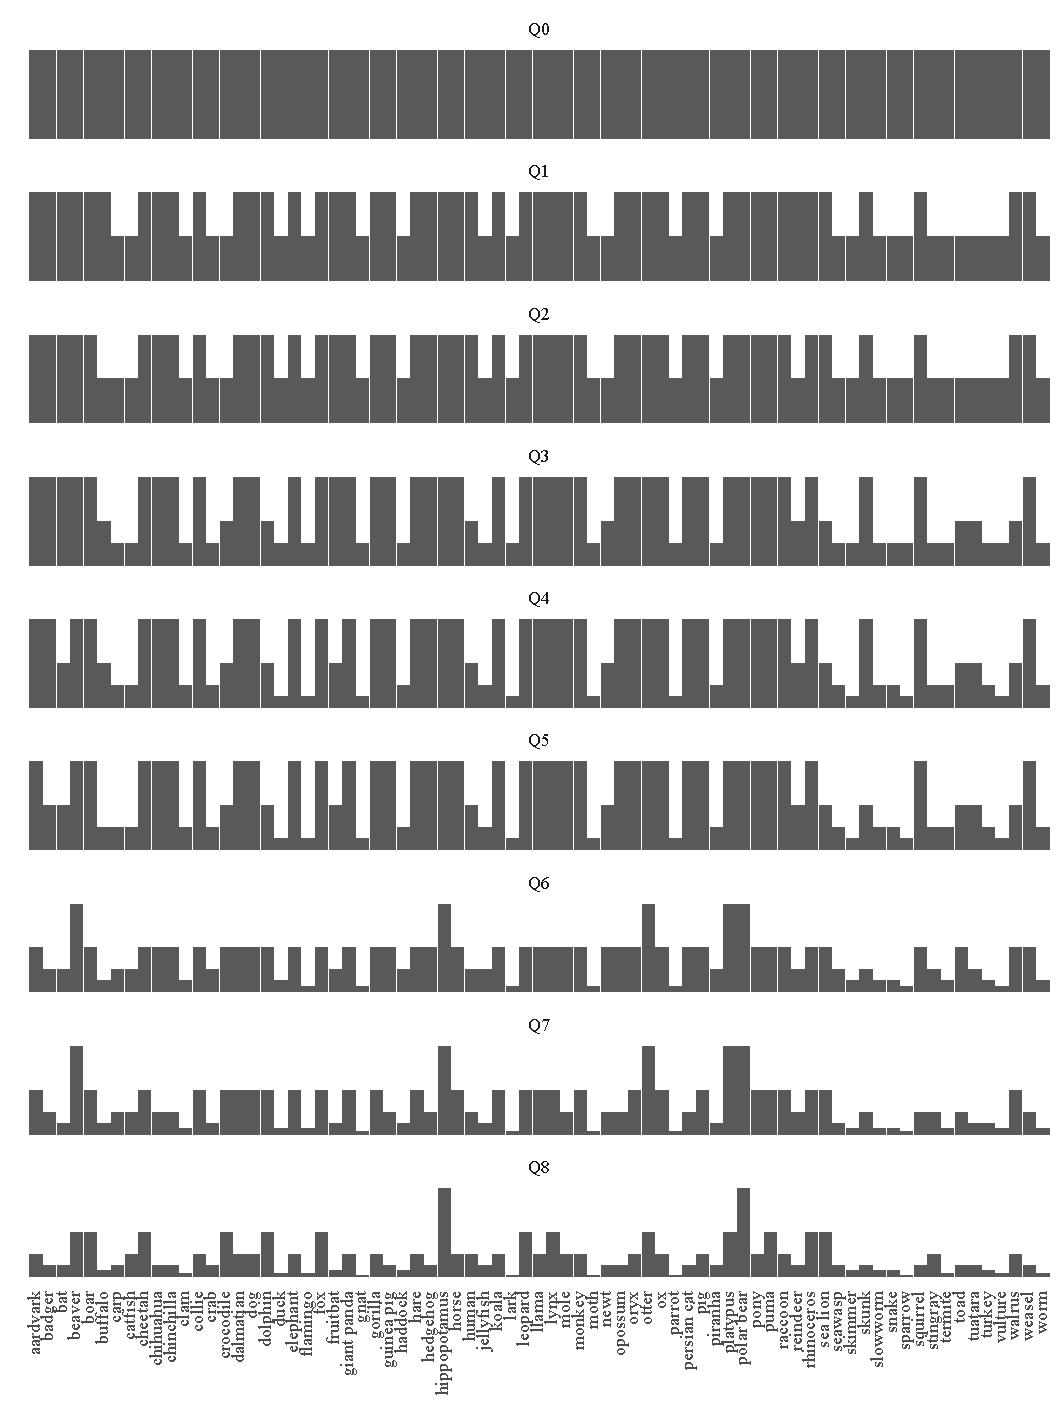
\includegraphics[width=\linewidth]{graphics/updating.pdf}
	\caption{Updating of probability scores across nine questions (only shown for a subset of 75 animals)}
	\label{fig:bayesian-update}
\end{figure*}

% ==============================================
\subsection{Guessing the animals}
\label{subsec:guess-animals}
% ==============================================

Eventually, the gameplay will reach a point when the remaining animals in the pared-down knowledge base can no longer be distinguished by any of the features, since all the features will contain all 0s or all 1s.
At this point, the game moves on to the stage of guessing the animals that the user may be thinking of.

We were inspired by the approaches of \citet{DeyEa2019}, \citet{HuEa2018}, and \citet{Burgener2006}, who all maintain a probability distribution over outcomes that is updated over the course of the game based on the answers that the user provides.

The motivation behind this approach, as we mentioned above, is to improve the flexibility of the system, and in particular to not reject outright any outcomes that are incompatible with the user's \mbox{answers}.
Instead of removing these from the pool of potential answers immediately, their probability is simply reduced, but this means that they are still ``in the running'' to be guessed by our system, after it has guessed the higher-probability items.

Technically, the distribution that we maintain over animals is not a probability, since it does not sum to one; rather, it is a probability score that keeps track of how (in)compatible each animal is with the answers that the user has provided so far.
It can be thought of as bargain-basement Bayesian updating.

We initialise a uniform prior probability score of 20 (an arbitrary choice) across all animals at the beginning of the game and update it after each question based on the user's answers.
Specifically, we divide the current probability for each animal in half (also an arbitrary choice) if it is incompatible with the answer the user just gave.
Once the features have all been used up, we have a distribution of probability scores across animals that reflect how compatible they are with the user's answers.
Figure \ref{fig:bayesian-update} illustrates how this distribution changes over the course of a game.

The animals that are perfectly compatible with everything the user has entered have the same probability score that they started with; those that are incompatible with only one answer have half of the prior score, and so on.
At the end of the game, the system guesses the animals in decreasing order of probability.
For the example shown in Figure \ref{fig:bayesian-update}, it would guess \texttt{polar bear} and \texttt{hippopotamus} (the only ones with a probability score of 20), followed by the animals with a probability score of 10, and so on.

% ==============================================
\subsection{Template-based question generation}
\label{subsec:qg}
% ==============================================

% TODO ELIZABETH: reformulate this entire section so it's more results-oriented

Now that we know which features or animals to ask about when, we come to the front-facing part of the system where questions about these entities are generated.
The QG section of this project consists of two sub-parts, namely

\begin{enumerate}
\item preprocessing the Switchboard Dialog Act Corpus (SwDA; \citealt{JurafskyEa1997,ShribergEa1998,StolckeEa2000}) to identify structures of polar questions,\footnote{The code used for preprocessing can be found here:  \url{https://github.com/epankratz/twenty-questions/blob/master/SWDA/swda_preprocessing.ipynb}.} and
\item feature-to-question generation. 
\end{enumerate}

We decided to work with the SwDA to be able to investigate the different structures of polar questions and to use those as a reference point for the questions we will generate.
Since the 20Q gameplay is based exclusively on the use of polar questions, which correspond to the tag \texttt{qy} in the SwDA, we extracted questions marked by this tag.
Then, we analyse the POS tags in these sentences, since the question templates we will use vary based on the POS of the variable element.
Table \ref{tab:swda_preprocessing} shows some examples of the question from the SwDA, its POS tagging there, and the POS tags from spaCy, which we have chosen to work with because of their simplified structure.%
	\footnote{We also tried performing NER on the feature names using spaCy, but this did not work on the out-of-context elements at all.}

\begin{table*}
\centering
\renewcommand{\arraystretch}{1.5}
{\small
\begin{tabularx}{\linewidth}{LLL} 
	\toprule
	Text & SwDA POS & spaCy POS \\ \midrule
	Were you -- & Were/VBD you/PRP --/: & \texttt{[`VERB', `PRON']}  \\
	Are you in Texas?/ & Are/VBP you/PRP in/IN Texas/NNP ?/. & \texttt{[`VERB', `PRON', `ADP', `PROPN']} \\
	I probably would |have done, \newline {D you know, } just… & I/PRP probably/RB would/MD have/VB done/VBN ,/... & \texttt{[`PRON', `ADV', `VERB', `VERB', `VERB', `NOUN'...]} \\
	 Are you a Vietnam veteran, Dudley? & Are/VBP you/PRP a/DT Vietnam/NNP veteran/NN ,/... & \texttt{[`VERB', `PRON', `DET', `PROPN', `NOUN', `PROP'...]} \\
	Do you have family who were in the Vietnam War? & Do/VBP you/PRP have/VB  family/NN who/WP were/V... & \texttt{[`VERB', `PRON', `VERB', `NOUN', `PRON', `VERB'...]} \\
	\bottomrule
\end{tabularx}
}
\caption{The first five rows of the SwDA dataframe, including the spaCy POS tags}
\label{tab:swda_preprocessing}
\end{table*}

The next step in the preprocessing was to remove uninformative POS tags such as \texttt{PUNCT} (punctuation) and \texttt{SPACE} (blank spaces).
Then, in order to investigate the general structure of polar questions, we concentrated on the first five POS tags in each sentence and counted the frequency of each POS tag sequence.
We ended up with 1332 unique POS tag sequences, the five most frequent of which are shown in Table \ref{tab:pos_patterns}.
The most frequent one, \texttt{(VERB, PRON, VERB, DET, NOUN)}, would for example correspond to a question like ``Does it have a tail?''.

\begin{table}
\centering
{\small
\begin{tabular}{lr}
	\toprule
	Count & POS tag sequence \\ \midrule
    153 & \texttt{(VERB, PRON, VERB, DET, NOUN)}\\
	90 & \texttt{(VERB, PRON)}\\
	74 & \texttt{(VERB, PRON, CCONJ, VERB, PRON)}\\
	69 & \texttt{(PROPN, VERB, PRON, VERB, DET)}\\
	61 & \texttt{(VERB, PRON, VERB)}\\
	\bottomrule
\end{tabular}
}
\caption{Unique POS tag patterns and their frequency counts, extracted from the SwDA Corpus}
\label{tab:pos_patterns}
\end{table}

In addition to the structures that we gathered from the SwDA, we chose to add one further twist and incorporate a subtype of polar questions: tag questions.
These are interrogative constructions formed by a main clause (i.e.\ anchor) and a peripheral question tag \citep{Bawden2017, Bonsignori2007, TottieEa2006}, e.g. 
\begin{gather*}
    \underbrace{\text{``You are happy,}}_{\text{anchor}}\ \underbrace{\text{aren't you?''}}_{\text{question tag}}. 
\end{gather*}

In a discourse, tag questions can have particular pragmatic power \citep{TottieEa2006}, and we are using them to indicate bias on the part of the 20Q player.
If the system chooses a feature, it might expect that the user's answer of whether their animal has that feature will be ``yes'' if most of the values for that feature are 1.
In that case, it might ask, say, ``Your animal is big, isn't it?'' with a tag question, rather than the neutral ``Is your animal big?''.
This would give the 20Q player a more human, playful voice, and introduce some variety to the question templates as a whole.

For each feature, we compute an extremeness value that symbolizes how out-of-balance the \mbox{values} for a given feature are.
If the extremeness value exceeds a certain threshold (which we set at 0.65), a biased question is chosen over the non-biased version.

We initially considered implementing not only positive-anchored biased questions, as in (\ref{ex:pos-tag}), but also negative-anchored biased questions, as in (\ref{ex:neg-tag}).

\enumsentence{Your animal \textit{is} big, isn't it?}\label{ex:pos-tag} 
\vspace{-1.25\baselineskip}
\enumsentence{Your animal \textit{doesn't have} feathers, does it?}\label{ex:neg-tag}

This would have been possible, but we realized that if negative-anchored biased questions like in (\ref{ex:neg-tag}) are answered affirmatively, ambiguities arise.
For example, it is unclear whether the answer ``yes'' to the question ``Your animal doesn't have feathers, does it?'' means that the animal indeed has feathers or that it does not.
Being faced with negative-anchored biased questions like this might confuse the human player, which would negatively affect the functioning of our system.
Therefore we opted to only include positive-anchored biased questions.

So, we now have question templates based on the POS tag of the variable element that are based on structures found in the SwDA, in both biased and unbiased versions (see Table \ref{tab:question_patterns}).
Notice that one question template, namely the biased question with a verb or auxiliary, requires that the verb or auxiliary be in the third person singular form in order make the question syntactically coherent. 
To take care of this, we made use of the \texttt{LemmInflect} library, a useful natural language processing library that can be used in combination with spaCy and that provides all inflectional forms for a given word.%
	\footnote{\url{https://github.com/bjascob/LemmInflect}; accessed 14.08.2020.}

\begin{table*}[ht]
\centering
	\begin{tabularx}{\linewidth}{lLL}
		\toprule
		POS tag & Unbiased & Biased \\
		\midrule
		\texttt{VERB} (+ed), \texttt{ADJ}, \texttt{ADV} & Is your animal \{feat\}? & Your animal is \{feat\}, isn't it? \\
		\texttt{NOUN} (pl), \texttt{DET}, \texttt{NUM} & Does your animal have \{feat\}? & Your animal has \{feat\}, doesn't it? \\
		\texttt{NOUN} (sg) & Is your animal a/an \{feat\}? & Your animal is a/an \{feat\}, isn't it? \\
		\texttt{VERB}, \texttt{AUX} & Does your animal \{feat\}? & Your animal \{feat.\textsc{3sg}\}, doesn't it? \\
		\texttt{ADP} & Does your animal live \{feat\}? & Your animal lives \{feat\}, doesn't it? \\ 
		\bottomrule
	\end{tabularx}
\caption{Question patterns based on POS tag of the first token in the feature name and bias status}
\label{tab:question_patterns}
\end{table*}

Now that the templates are in place, the QG proceeds according to the following steps.

\begin{enumerate}
  \item Preprocessing and tokenising the feature names, i.e.\ changing underscores to spaces and tokenising the string in a format that can be POS-tagged.
  \item POS-tagging of the first word in the feature string using spaCy's \texttt{pos\_} method.
  \item Generating a question by choose one of the pre-defined question patterns depending on the extremeness value of the feature and the POS tag obtained in the previous step.
\end{enumerate}

We did face some challenges with Step 2 during development.
Specifically, spaCy's POS tagger didn't correctly tag all of our features, resulting in some ungrammatical questions.
For instance, it would only tag the feature \texttt{fly} as a noun, not a verb, and \texttt{nocturnal} as a proper noun, for some reason, and not an adjective.
We also tried WordNet's POS tagger \citep{Fellbaum2010}, but it still had poor accuracy with our feature names. 
Presumably, these problems can be attributed to the fact that we used out-of-context tagging.

We ultimately decided that the best solution would be to simply rename the mis-tagged features (e.g.\ changing \texttt{fly} to \texttt{the ability to fly}, giving ``Does your animal have the ability to fly?'', and \texttt{nocturnal} to \texttt{active mainly at night}, giving ``Is your animal active mainly at night?'').

% ==============================================
\subsection{Incorporating out-of-database objects}
\label{subsec:out-of-db}
% ==============================================

Before concluding the implementation section, we turn to our last challenge: successfully incorporating out-of-database objects into our knowledge base. 
We adopted a strategy inspired by the following quote:

\begin{displayquote}
The perceived world is not an unstructured total set of equiprobable co-occurring attributes. 
Rather, the material objects of the world are perceived to possess ...\ high correlational structure.
That is, given a knower who perceives the complex attributes of feathers, fur, and wings, it is an empirical fact provided by the perceived world that wings co-occur with feathers more than with fur. \citep[29]{Rosch1978}
\end{displayquote}

Following this logic, for animals that are not in our knowledge base, we can exploit the correlations between similar animals to expand our knowledge base and improve the system over time.
Every time the 20Q player loses, the human player is asked to give the name of the animal they were thinking of. 
If said animal is not already in the knowledge base, a new entry will be created for it, and the features that were asked about will be populated with the user's input. 
The system can gather at most 20 features for each animal, since it can ask at most 20 questions, which means that it will need to fill in the 43 or more empty fields in the new entry itself.
This is where the interpolation of unknown features comes in.

To fill in these empty values, we decided to work with two correlation methods. 
Our goal was to find the most highly correlated animal to the out-of-database target (given the user's input) and subsequently populate the empty fields with the values from the highly-correlated animal's entry in the knowledge base. 
For example, given \textit{coyote} as an out-of-database object, one would expect it to have many shared features with an animal like \textit{wolf}. 
Our aim in these similarity measures is to find the existing animal in the knowledge base that most closely matches the user's input and therefore is likely a similar animal.

When initializing the 20Q game, the human user is given the option of specifying which correlation method to be used to interpolate any out-of-database objects. We will discuss the two methods in detail in the present section.

The first correlation method takes \citeauthor{Rosch1978}'s \citeyearpar{Rosch1978} words to heart, tallying the total number of features that a pair of animals has in common. Although this method is very simple, it often generates similar animals that are very close to human intuitions. We called this method \texttt{OURS}. 
The second method, which we called \texttt{CORR}, computes a pairwise Pearson correlation coefficient between the out-of-database animal and each remaining animal. 
The performance of these two methods are evaluated in Section \ref{subsec:eval-interpolation} below.

\begin{figure*}[htbp!]
\centering
	
\includegraphics[width=.9\linewidth]{graphics/call_graph.pdf}
	\caption{Call graph of non-utility class methods in \texttt{TwentyQuestions}. Methods in (1) are for sampling features; (2) for asking users about features, getting user input, and taking the respective action; (3) for guessing animals; and (4) for the endgame and adding out-of-database animals}
	\label{fig:call-graph}
\end{figure*}

Having discussed our strategy for handling cases in which the target animal is not in the knowledge base, we turn now to our strategy for games that were lost by the 20Q player but for which the target animal was, in fact, in the knowledge base. 
In these instances, we still add a new row for the animal to preserve the human player's answers, but instead of using a correlation method, we fill the empty cells with the values from the animal's existing row in the knowledge base. 
The result is two entries for the given animal in the knowledge base, one with the newly-acquired human judgments and another with more factual information. 
As we discussed in class, 20Q is a game in which it's more interesting to note what the players \textit{think} about animals, even if this deviates from what is actually true. 
In this way we are able to capture both the objective information and more subjective, human judgment. 
In order to prevent the system from guessing the same target animal more than once in a single game, we implemented a check in the gameplay code to ensure that each animal name could only be guessed one time (only the highest-probability instance of each animal is guessed).  

\vspace{\baselineskip}

\noindent The call graph in Figure \ref{fig:call-graph} provides a visual summary of how the (non-utility) methods in the \texttt{TwentyQuestions} class fit together.

% ==============================================
\section{Evaluation}
\label{sec:eval}
% ==============================================

We evaluated two aspects of the performance of our 20Q player. 
The first, as one might expect, was the win and loss rate of our system over time. 
The second was how well our player could interpolate from the existing knowledge base entries to fill in missing data for newly-added animals.
We discuss these aspects in detail below.

% ==============================================
\subsection{Win/loss rate}
\label{subsec:eval-win-loss}
% ==============================================

Before we could calculate our system's win/loss rate, we first had to play enough games to have meaningful statistics. 
All group members played against our system with the same 24 target animals: twelve randomly-selected in-database target animals and twelve out-of-database animals. 
The intuition behind this choice was that the system would learn about the out-of-database animals from the first player's inputs and interpolate values for the features that weren't asked about in the game. 
For an out-of-database animal that had never been introduced before, the system would be able to gather information about features of that new animal, which could then be utilized by the interpolation measure to fill in the remaining feature values. 
For subsequent games, then, the system would have this new animal in its knowledge base and would have the opportunity to guess it correctly. 

As expected, for the first two players who played with the out-of-database animals, the system could not guess them correctly.
However, by the third and fourth plays for the out-of-database targets, the system was able to win a game for six of the twelve newly-introduced animals.
Interestingly, even if the system managed to guess an out-of-database animal for one player, it often was unable to win again on the same animal for the next player.
We speculate that this may be due to the interaction of our random question selection and our interpolation measures. 
It could be the case that the human player's answers are incompatible with the interpolated data, and thus the probability distribution would be biased away from the correct target animal. 
However, after a significant number of plays, we expect that the system would be able to gain enough information to improve its win rate for these items as well.

At the time of writing, our model had logged 94 total plays. 
Although this is not a large number from a statistical standpoint, it is enough to allow us to do some analysis and assess how the model might be expected to improve over time. 
Of these 94 plays, 40.4\% were wins and 59.6\% were losses. 
The losses can be categorized into two types: those for which the animal was in the database but not guessed within 20 questions, and those due to out-of-database items. 
Of the losses, 78.5\% were of Type 1, and 21.5\% were of Type 2. 
Figure \ref{fig:wins-losses} illustrates these results. 

\begin{figure}
    \centering
    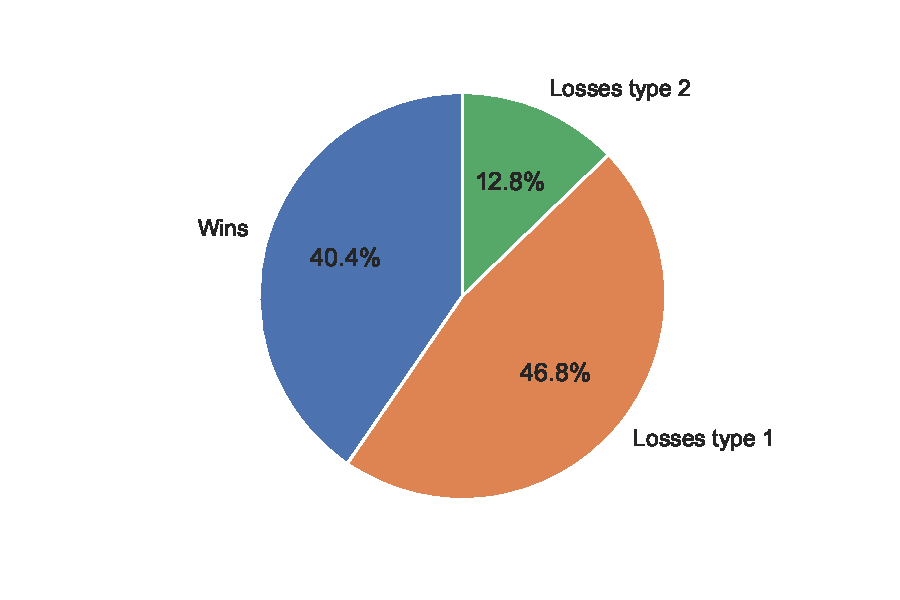
\includegraphics[width=\linewidth]{graphics/pie_detailed-winsLosses.pdf}
    \caption{The win/loss rate after 94 games; Type 1 losses are losses on in-database items, and Type 2 losses are losses on out-of-database items}
    \label{fig:wins-losses}
\end{figure}

We plotted the win/loss rate over time to see how it evolved with respect to the number of games played. 
Although our total number of plays is too low to give us an accurate picture of how the 20Q player would perform after many more plays, it seems reasonable to expect an upward trend (see Figure \ref{fig:win-over-time}).

\begin{figure}
    \centering
    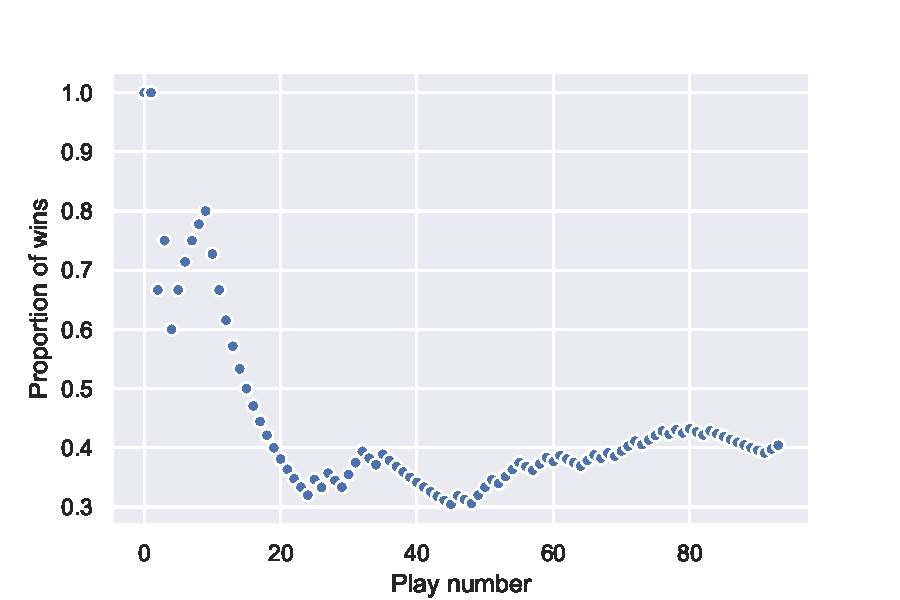
\includegraphics[scale = .5]{graphics/stats-eval.pdf}
    \caption{The proportion of wins to losses show an increasing tendency over time}
    \label{fig:win-over-time}
\end{figure}

% ==============================================
\subsection{Quality of interpolated out-of-database items}
\label{subsec:eval-interpolation}
% ==============================================

Recall from Section \ref{subsec:out-of-db} the two methods for filling in the unknown features of out-of-database animals: \texttt{OURS} counts the number of features that a pair of animals shares, while \texttt{CORR} computes a pairwise Pearson correlation coefficient between the features of a pair of animals.
We compare these methods in two ways.
First, we look at how comparable their similarity rankings of animals in the database are. 
Second, we consider how similar the values that each method interpolates are to a gold standard.

\subsubsection{Similarity rankings}

Our aim was to see how comparable the two methods are in the animals that they consider to be similar.
To this end, we hand-selected seven pairs of animals that common sense would deem highly correlated.
We then removed one first animal in each pair from the database and reintroduced it as an out-of-database item. 
Running both methods on the now-out-of-database animal, we generated the top five most similar animals.%
    \footnote{The code used for evaluating the similarity measures can be found here: \url{https://github.com/epankratz/twenty-questions/blob/master/code/Sim_comparison.ipynb}.}

Two of the most interesting results can be found in Tables \ref{tab:corr1} and \ref{tab:corr2}.
For the pair (\textit{dog}, \textit{German shepherd}) in Table \ref{tab:corr1}, the \texttt{OURS} method returned animals that match quite nicely with human intuition, performing far better than the \texttt{CORR} method, which returned animals that are very different both from \textit{dog} and from each other.%
    \footnote{In the Jupyter Notebook, \textit{deer} is given as number 5 for \texttt{CORR}.
    \textit{dog} is substituted here for illustrative purposes because it received the same score, but appears lower alphabetically.}
We speculate that this may be due to the overly general nature of the object \textit{dog}, which, given our decision to assign 1s to features for which one might answer with either yes or no, as we discussed in Section \ref{sec:knowledge-base}, shares features with a wide range of different animals.

However, turning to the pair (\textit{chimpanzee}, \textit{monkey}) in Table \ref{tab:corr2}, we see that both correlation measures returned the same animals in the same order. 
This is promising and shows that both methods do a fair job at pinpointing similar animals in a way that is (usually) similar to human judgments.

\begin{table}[]
    \centering
    \begin{tabular}{clcclc}
    \toprule
    & \multicolumn{2}{c}{\texttt{OURS}} && \multicolumn{2}{c}{\texttt{CORR}} \\
    \cmidrule{2-3} \cmidrule{5-6}
    1. & collie & 61 && cockroach & 0.92 \\
    2. & dalmatian & 59 && chicken & 0.84 \\
    3. & chihuahua & 59 && crow & 0.84 \\
    4. & raccoon & 59 && raccoon & 0.84 \\
    5. & dog & 58 && dog & 0.83 \\
    \bottomrule
    \end{tabular}
\caption{Correlation scores for \textit{German shepherd} as the out-of-database item and \textit{dog} as in-database reference}
\label{tab:corr1}
\end{table}

\begin{table}[]
    \centering
    \begin{tabular}{clcclc}
    \toprule
    & \multicolumn{2}{c}{\texttt{OURS}} && \multicolumn{2}{c}{\texttt{CORR}} \\
    \cmidrule{2-3} \cmidrule{5-6}
    1. & gorilla & 59 && gorilla & 0.81 \\
    2. & baboon & 58 && baboon & 0.74 \\
    3. & human & 57 && human & 0.73 \\
    4. & wallaby & 57 && wallaby & 0.70 \\
    5. & baboon & 57 && baboon & 0.70 \\
    \bottomrule
    \end{tabular}
\caption{Correlation scores for \textit{chimpanzee} as the out-of-database item and \textit{monkey} as in-database reference (\textit{monkey} was scored 56 by \texttt{OURS} and 0.69 by \texttt{CORR})}
\label{tab:corr2}
\end{table}

\subsubsection{Accuracy of interpolated features}

To test the quality of the interpolation for the out-of-database items, we randomly selected twelve animals from the knowledge base to serve as a gold standard.
Then, one at a time, we removed each animal from the knowledge base and played a game in which the system was made to guess the (now-missing) animal. 
Of course, it will not be able to guess the animal, since it is no longer in the knowledge base.
Our goal is to see how close the system's interpolations are to the true values for that animal, and whether the accuracy of interpolation varies greatly between the two similarity measures \texttt{OURS} and \texttt{CORR}.

For \texttt{OURS}, the mean accuracy rate of the interpolation across all animals was 82.1\%, i.e.\ the system interpolated the correct value in 82.1\% of cases.
And for \texttt{CORR}, the mean accuracy rate of the interpolation was 77\%.

Figure \ref{fig:interp-eval} suggests a weakly positive correlation between the number of features that were asked about and the accuracy of the interpolations, which makes sense.
The more features that the user provides, the more information the system can use to make an educated guess about the remaining features.


\begin{figure*}
\centering
\begin{tabular}{@{}ccc}
\texttt{OURS} && \texttt{CORR} \\
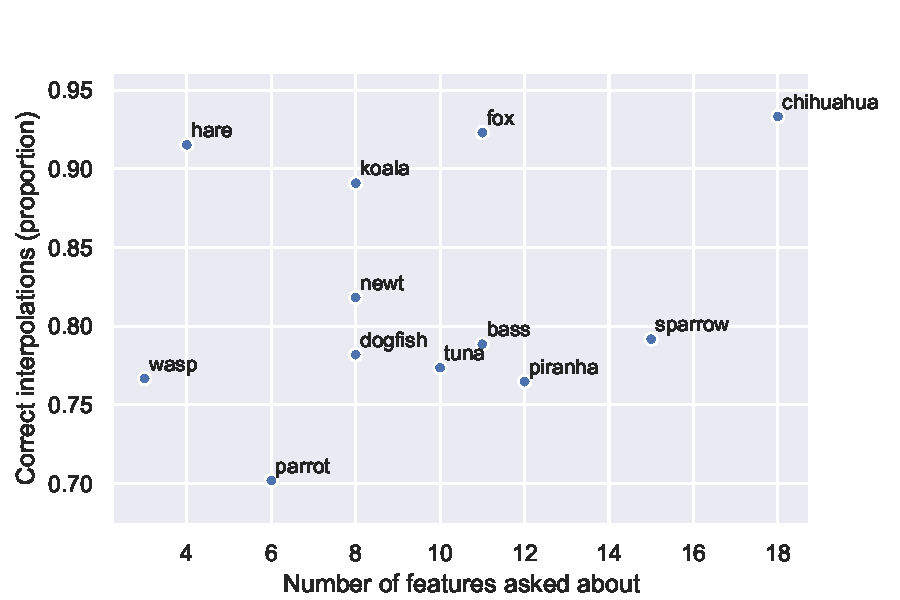
\includegraphics[trim=0 0 0 30,clip,width=.48\linewidth]{graphics/interpolation-eval-ours.pdf} && 
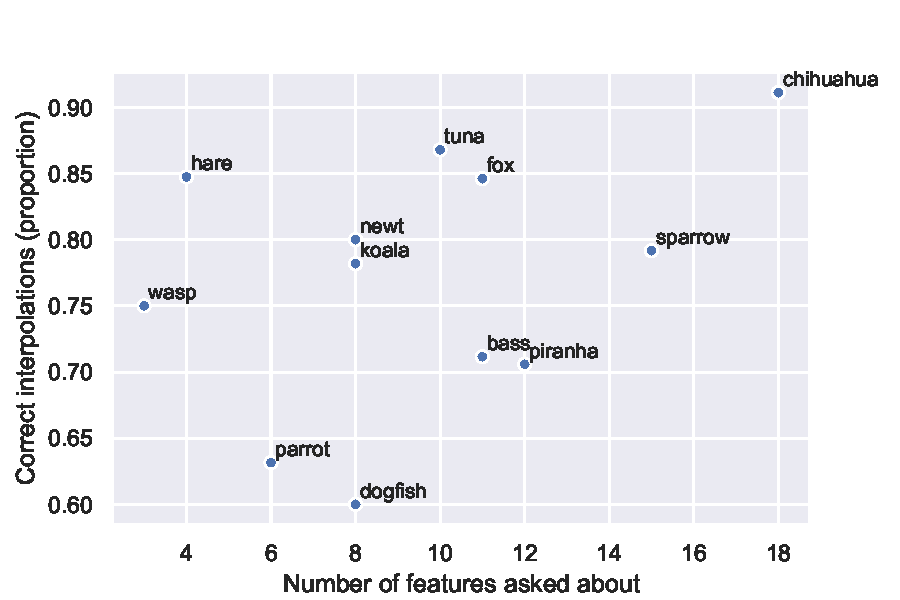
\includegraphics[trim=0 0 0 30,clip,width=.48\linewidth]{graphics/interpolation-eval-corr.pdf} \\
\end{tabular}
	\caption{For both similarity measures, the proportion of correctly interpolated features shows a weakly positive correlation with the number of features the system asked about}
	\label{fig:interp-eval}
\end{figure*}

% ==============================================
\section{Limitations of our system}
\label{sec:limit}
% ==============================================

There are several aspects of our system that could be improved upon in future work. 
Although we did implement some strategies to better handle games with so-called ``noisy input'', in which a user's answers did not exactly match the entry for the target animal in our knowledge base (for instance, accepting ``unknown'' as an answer, ranking features by their relative objectivity, and the probability distribution, as discussed above), our model's performance in such cases still has room for improvement. 

Our feature selection method is such that the game may not be asking questions that will lead to the correct animal being guessed. 
Because the feature selection method chooses the best feature for the remaining partition of the knowledge base, if the target animal is not in that partition (i.e.\ if the user's input was incompatible with the knowledge base's representation of that animal), the system's questions are biased away from the target animal. 
The probability score distribution across animals is a strategy we implemented to address this problem, but it is still less likely that the correct animal will be guessed.

Another limitation of our system, as alluded to in Section \ref{sec:litreview}, is the set of answer inputs available to the human player. 
While the current iteration of our 20Q game only allows for inputs of 0, 1, and 2 for ``no'', ``yes'', and ``unknown'', respectively, an avenue for future work would be to incorporate a wider range of answer choices, as in \citet{Burgener2006}'s implementation. 
Adding inputs that are less black and white than a binary split (for instance, ``I think so'', ``I don't think so'', ``sometimes'', or ``it's possible'') would make the game easier to play and positively impact the probability distribution, perhaps leading to a higher win rate. 

Admittedly, our feature selection system does not learn to ask better questions over time; the method of choosing the best feature to ask about at a given time does not follow a strategy that extends beyond each individual turn. We chose to focus our efforts on other parts of the project instead, since the current strategy already works fairly well.

If we were to develop the system further, though, this would certainly be a point of improvement, e.g. by learning from previous games which sequences of questions tend to perform well. This approach would also ostensibly rectify another limitation of our system, namely that questions that should be mutually exclusive: if a user answers ``yes'' to the question ``Does it have four legs?'', the system need not subsequently ask if the animal has two legs. 

Another potential point of improvement concerns the questions we generated.
For future projects, it would be interesting to perform POS-tagging in combination with NER on in-context elements in consonance with \citet{Mandasari2019}, which seems like a promising approach that would yield correctly-analyzed named entities that could be fitted into question templates without further preprocessing. 
We would also be interested to try a rule-based approach for QG, by developing a question template composed of syntactic categories to be filled later on, or to work with a more complex linguistic architecture. 

Recall also from Section \ref{sec:knowledge-base} that instances where the feature could be ambiguous, such as those related to color and size, were marked with 1 to capture the fact that the given feature \textit{could} be said to be true for the target.
Future iterations might modify the question template for this subset of features to reflect this sense of possibility or uncertainty.

Finally, our interpolation measures could be more sophisticated. While our measures perform relatively well, as discussed in section \ref{subsec:out-of-db}, our system could be improved by adopting an interpolation method that could take into account feature data for more than one animal. 
Another approach could focus more on the features themselves than the animal, giving relative likelihoods of one feature given another.
Furthermore, since the interpolation tends to match the gold standard more closely when more questions have been asked, we could engineer the system to recognise that it will probably not guess the user's animal and, in that case, to ask as many probing questions as possible, to get more information that will improve the quality of its guessing.

% ==============================================
\section{Conclusion}
\label{sec:concl}
% ==============================================

Our fairly humble 20Q system may not hold its own against the top players on the market, but in working on this project we have taken on tasks that are both engineering-oriented and linguistic in nature and have learned a lot about question generation, manipulation of knowledge bases according to the provided answers, and (not least) how to work in a team. 

% ==============================================

\bibliography{qp}
\bibliographystyle{acl_natbib}

\appendix

% ==============================================
\section{Individual contributions}
\label{app:contributions}
% ==============================================

All group members were in regular, active communication about ideas and directions in which to take the project.
It was a fully collaborative effort throughout.
We summarise here how we divided the workload between the four of us.

\paragraph{Wellesley} Literature work, prepared and held the in-class presentation, created the knowledge base, wrote and proofread sections of the project plan and the final paper.

\paragraph{Anna} Literature work, implemented the question generation, wrote sections of the project plan and the final paper.

\paragraph{Rodrigo} Implemented the handling of out-of-database items, evaluated performance of the system and handling of out-of-database items with \texttt{CORR}.

\paragraph{Elizabeth} Implemented the \texttt{TwentyQuestions} class and its core methods, wrote and proofread sections of the project plan and the final paper, evaluated handling of out-of-database items with \texttt{OURS}, created graphics.

\end{document}
